\section{文献综述与技术依据}

本章的目的不是提前重复后续实现细节，而是说明这些方法选择从何而来。
围绕 Mie 几何观测量、短脉冲穿深行为、多孔喷油束配准、右删失目标、
不确定性感知代理模型和概率性撞壁风险筛查，本文梳理既有研究能够提供的支撑，
也指出尚未被单一文献脉络完整覆盖的问题。
这一章因此承担的是承上启下的作用：
在进入具体工作流之前，先把既有知识与本文工程设计决策之间的逻辑链条交代清楚。

\subsection{面向跨学科读者的方法学术语简介}\label{sec:methods-terminology}

本文的实现跨越四个技术领域：计算机视觉、数值优化、GPU 并行计算与深度学习。
这四类工具在本文中依次衔接：图像处理从视频中提取穿深观测量；
鲁棒优化将含噪轨迹压缩为稳定的拟合目标；
GPU 并行使大批量处理能在合理时间内完成；
神经网络则从这些目标中学习条件预测分布。
对于以流体力学与机械设计为主要背景的读者，本节先就各领域中最少必要的概念给出直观说明，
以便后续章节中的技术选择可被理解为工程决策，而非难以解读的黑箱。

\textbf{计算机视觉与信号处理。}
计算机将图像存储为数值矩阵：每个像素对应矩阵中的一个元素，其数值表示该点的强度或亮度。
对图像的处理本质上即对该矩阵施加数学运算。
\emph{卷积} 是最基本的运算：一个小型模板窗口（卷积核）逐像素滑过图像，每一步执行一次加权求和。
其效果取决于核的形状，可用于平滑图像、提取边缘或增强纹理。
Sobel 算子是一种用于计算局部亮度梯度（变化率）的卷积核，
对液相边界一类的对比度突变响应最强，因此是喷雾图像中边界定位的标准工具。
\emph{极坐标变换} 将图像由直角坐标（像素行列）转换为以角度和径向距离为轴的坐标系。
围绕已校准的喷嘴中心进行该变换，可将多孔喷雾的方向结构折叠为一维角度信号，从而显著简化后续配准。
\emph{快速傅里叶变换}（FFT）将信号分解为不同频率的正弦分量，
将周期结构直接暴露为频域峰值；本文借此自动识别多孔喷雾的旋转周期性，进而估计各喷孔的角度偏移。

\textbf{鲁棒优化与曲线拟合。}
最小二乘拟合的几何含义是寻找一条曲线，使所有观测点到该曲线的距离平方和最小。
当数据中含少量离群点（如受光学噪声污染或带有少量量化误差的帧）时，
平方型惩罚会让这些点对结果产生不成比例的影响。
Huber 损失是一种折中：残差较小时保留平方惩罚的光滑性，
残差超过阈值后切换为绝对值惩罚，从而抑制离群点的杠杆效应——
这与测量实践中``舍弃异常读数''的工程直觉完全一致，并具有坚实的稳健统计学基础 \cite{Huber1964,NocedalWright2006}。
神经网络训练所用的 \emph{梯度下降} 算法在当前参数处计算损失对各参数的偏导数，
然后沿最陡下降方向微调参数，直到损失不再显著减小——
概念上等价于在高维参数空间中迭代地``沿坡而下''。

\textbf{GPU 并行计算。}
CPU 通常拥有少量经过深度优化的核心，擅长处理复杂的串行逻辑任务；
GPU 则拥有数千个较简单的核心，适合对大量结构良好的数据元素同时施加相同的算术运算。
图像处理恰好契合这一模式：对每个像素进行卷积、对每个角度区间累加、对每帧进行阈值化——
这些操作在像素或帧之间完全独立，GPU 可以将其真正并行地分发到数千个核心上同时执行。
CUDA 是 NVIDIA 提供的并行计算平台；
CuPy 是与 NumPy 接口兼容的 Python 库，使本文的图像处理链能以最小的代码改动切换至 GPU 后端。
GPU 加速的工程意义在于：将 TB 级视频归档的批处理由``需若干天''转变为``若干小时内完成且支持迭代细化''，使整个研究流程真正具备可循环性 \cite{NickollsBuckGarlandSkadron2008}。

\textbf{神经网络与深度学习。}
本文使用的神经网络为多层感知机（MLP）：
若干层线性变换与非线性激活函数级联，构成一个具有可调参数的非线性函数；
以工况特征和时间为输入，输出穿深预测。
深层网络还需要适当的正则化与优化策略。
例如，随机单元屏蔽（Dropout）在训练期间随机丢弃部分神经元，迫使网络学习冗余表示，从而降低稀疏工况支持下的过拟合风险 \cite{Srivastava2014Dropout}；
解耦权重衰减（Decoupled Weight Decay，如 AdamW）将权重衰减项从自适应梯度更新中分离出来，有助于改善泛化能力 \cite{LoshchilovHutter2019AdamW}；
平滑门控激活函数（如 SiLU/Swish）则保持网络导数的平滑传递，这对于后续实施物理导数惩罚尤其重要 \cite{Ramachandran2017Swish}。
参数通过训练得到——在大量样本上反复计算预测误差，并以梯度下降迭代更新权重，直至总体误差收敛。
均方误差（MSE）是最简单的训练目标，对应条件均值回归。
异方差高斯负对数似然（NLL）是其扩展：网络同时输出条件均值与条件方差，
等价于为每个工况点提供一条随条件变化的误差带宽，而非对所有条件使用同一固定误差带 \cite{KendallGal2017}。
知识蒸馏是一种师生训练框架：先训练一个在干净数据上表现良好的``教师''网络，
再训练``学生''网络，使其在数据稀疏或不完整的区域模仿教师的输出，
而非强行拟合缺失标签——类似于在样本不足时由经验丰富的工程师为初级工程师提供判断基线 \cite{HintonVinyalsDean2015}。

\subsection{Mie 散射成像原理与几何观测量}

Mie 散射被广泛用于致密液相喷雾可视化，一个重要原因在于其实验实现相对简洁；
与许多替代诊断手段相比，Mie 成像更易与高速摄影平台结合，从而获得较高时间分辨率 \cite{Linne2013SprayImaging}。
然而，成像实现相对容易并不意味着定量解释同样直接。
Mie 成像记录的是散射强度场，该信号不能直接等同于燃料质量或液体体积分数。
其散射响应取决于液滴尺寸、折射率、波长和观测几何；在致密区域中，多重散射和阴影效应还会进一步改变图像强度分布 \cite{BohrenHuffman2004,Linne2013SprayImaging}。
因此，试图由像素强度直接反演完整喷雾物理状态，本质上是一个不适定问题。

不同光学诊断方法对喷雾信息的响应机制不同。
DBI 通过背光消光表征路径积分光学厚度，通常适合提取液相轮廓；
Shadowgraph 与 Schlieren 主要响应折射率或密度梯度，更适合观察气相喷雾、边界不稳定性和破碎过程；
LIF 通过燃料或示踪剂荧光表征蒸汽分布或当量比；
PIV 关注速度场与湍流结构；
PDPA 则提供局部液滴粒径与速度信息。
这些方法均具有各自价值，但对于本文关注的非蒸发、非反应液相柴油喷雾而言，它们与目标观测量的匹配程度并不相同：
LIF、PIV 和 PDPA 更偏向组分、流场或单点粒径速度测量，难以直接支撑本文所需的高时间分辨率液相包络追踪；
Schlieren 与 Shadowgraph 虽可提供喷雾外形信息，但对液相边界的针对性不如液滴散射类方法明确；
DBI 与 Mie 则更接近本文关心的液相轮廓、穿深与锥角提取任务 \cite{Linne2013SprayImaging}。

这一定位与既有研究保持一致。
早期在光学柴油机内部进行的二维 Mie 散射工作即将射流尖端穿深与锥角作为图像分析的实用输出，
而非追求完整液相状态重建 \cite{MuenchLeipertz1992}；
即便在仪器水平和同步精度更高的近期成像研究中，液相喷雾比较仍围绕穿深和扩展角度量展开 \cite{JungManinSkeenPickett2015}。
这意味着以 Mie 视频为基础的研究，应首先以其所提取观测量的质量、可重复性与明示边界进行评判。

本文使用的数据来自 Wärtsilä OSCC 已完成的顶视多孔喷嘴 Mie 散射实验，而非在多种诊断方案中重新择优采集得到。
与常见的背光、侧视、单孔隔离布置相比，该实验通过侧向窗口照明，并将喷油器布置于舱体背面，使单次成像能够同时覆盖全部喷油束。
这一布置更适合保留本文后续建模所需的 plume-to-plume 与 shot-to-shot 差异。
基于上述方法属性，本文不将像素强度解释为可直接反演的热力学真值，而是将其作为液相边界的几何线索；
图像处理目标也被明确限定为提取穿深、锥角、投影面积和边界位置等操作性观测量。
其中，穿深是后续轨迹拟合、代理模型建模与撞壁风险筛查的核心输入 \cite{Linne2013SprayImaging,LefebvreMcDonell2017,Dent1971Penetration,HiroyasuArai1990,NaberSiebers1996}。
在这一定位下，靠近喷嘴处由多重散射造成的缓变光晕不被解释为局部液相浓度，而被视为需要在后处理中抑制的背景成分。

Mie 成像还带有一个特征性的多重散射物理限制：
在喷嘴附近的致密液核区域，反复散射和内部阴影使局部强度升高，但几乎不贡献清晰的方向结构，
因而产生弥散光晕而非清晰的喷雾边界 \cite{BohrenHuffman2004,Linne2013SprayImaging}。
本文将该光晕视为缓变背景成分而非局部液相浓度，相应的抑制方法（梯度域滤波）与视线积分下的几何修正归入第~3 章图像处理工作流中讨论。

需要进一步强调的是，从 Mie 强度场到几何观测量的过程依赖具体的测量规则。
Magnotti 和 Genzale 指出，不同液相穿深度量会在柴油喷雾模型验证中导向实质不同的结论，因为不同观测量响应的是底层液相分布的不同侧面 \cite{MagnottiGenzale2013}。
这意味着报告的``穿深''并非普适真值，而是特定测量规则作用于光学信号后的结果。
Engine Combustion Network（ECN）的基准研究为这种方法依赖性提供了系统证据：
ECN 在多个机构测试名义上相同的喷油器（Spray~A 和 Spray~D），发现液相穿深在不同设施和后处理定义之间存在可观测差异，并明确将光学液相边界界定为由特定测量协议定义的量，而非液相真实分布的绝对表示 \cite{ecn_liquid_penetration,ecn_liquid_penetration_accessory,MeijerECN2012}。
本文实验条件不同于 ECN Spray~A 的高温高压蒸发条件，也不同于 Spray~D 的基准设置：
本文使用的是室温加压环境下的多孔海用喷嘴顶视图数据，且不涉及燃油蒸发。
但 ECN 的方法论原则仍然适用：
穿深和边界数值依赖后处理规则，这一依赖必须进入结果解释。

\subsection{喷嘴瞬态穿深物理的经验模型及其局限}

传统喷雾经验模型长期围绕穿深展开，原因在于穿深能够将复杂喷雾演化压缩为少量具有物理意义的低阶量。
在 Hiroyasu--Arai 框架中，尖端穿深通常采用分阶段经验表达：破碎前近似随时间线性增长，破碎后则转为平方根标度，其简化形式可写为
\[
S_{\mathrm{tip}}(t)\propto
\begin{cases}
t, & t<t_b,\\
t^{1/2}, & t\ge t_b,
\end{cases}
\]
其中 \(t_b\) 为破碎时间，比例系数由压差、喷嘴直径和流体性质共同决定 \cite{HiroyasuArai1990}。
若把这一比例式写成本文基线实际采用的可拟合函数，则 Hiroyasu--Arai 基线可表示为
\[
S_{\mathrm{HA}}(t)=
\begin{cases}
k_v \left( \dfrac{2\Delta P}{\rho_l} \right)^{1/2}t,
& t<t_b,\\[6pt]
k_p \left( \dfrac{\Delta P}{\rho_a} \right)^{1/4}(d_n t)^{1/2},
& t\ge t_b,
\end{cases}
\qquad
t_b=k_b\,\frac{\rho_l d_n}{(\rho_a\Delta P)^{1/2}} .
\]
这里 \(d_n\) 是喷孔直径，\(\Delta P=P_{\mathrm{inj}}-P_{\mathrm{ch}}\) 是喷射压差，\(\rho_l\) 和 \(\rho_a\) 分别为燃油与环境气体密度。
在文献中，\(k_v\)、\(k_p\) 和 \(k_b\) 可取经验常数；在本文结果章的基线对比中，则将这三个无量纲系数在训练划分上重新标定，使该经验式在当前 OSCC 图像数据上获得公平的最佳表现。
该函数的物理含义很清楚：破碎前由喷孔出口速度控制，破碎后由动量通量、环境气体密度和喷孔尺度共同控制。

Naber--Siebers 关联式保留了类似的动量缩放，但更强调环境气体密度和喷雾扩散角对穿深的影响 \cite{NaberSiebers1996}。
在本文作为基线实现时，为避免引入无法在所有样本上可靠观测的角度先验，采用的是带时间延迟的降阶形式
\[
S_{\mathrm{NS}}(t)
=
k_{\mathrm{NS}}
\left(\frac{\Delta P}{\rho_a}\right)^{1/4}
d_n^{1/2}
\left[\max(t-\tau,0)\right]^{1/2},
\]
其中 \(k_{\mathrm{NS}}\) 为拟合增益，\(\tau\) 为有效起始延迟。
若使用完整角度修正，扩张角 \(\alpha\) 可通过近似因子 \((\tan(\alpha/2))^{-1/2}\) 改变同一动量尺度；
但本文报告的 Naber--Siebers 基线不使用训练集锥角或 oracle 锥角，而只拟合 \(k_{\mathrm{NS}}\) 与 \(\tau\)，从而保持与其他模型相同的输入可用性。

第三类参照不是封闭形式喷雾物理式，而是 Gaussian process（GP）非参数回归基线 \cite{RasmussenWilliams2006}。
它把穿深或缩放穿深视为由输入特征驱动的随机函数，
\[
f(\mathbf{x})\sim\mathcal{GP}\!\left(m(\mathbf{x}),\,K(\mathbf{x},\mathbf{x}')\right),
\qquad
S(\mathbf{x})=A\,f(\mathbf{x}),
\]
其中 \(A=(\Delta P/\rho_a)^{1/4}d_n^{1/2}\) 是上文同一 Hiroyasu--Arai 破碎后幅度，\(\mathbf{x}\) 包含时间、喷束倾角、喷孔数、喷射持续时间和控制背压等经过标准化的特征。
GP 的可调对象不是少数物理系数，而是核函数超参数：幅度、长度尺度、噪声水平，以及在自动相关维度（ARD）设置下各输入维度各自的长度尺度。
本文的稀疏异方差 GP 基线进一步用一个均值 GP 和一个对数残差方差 GP 共同给出 \(\mu_S(t)\) 与 \(\sigma_S(t)\)，并通过稀疏变分近似扩展到大样本表 \cite{HensmanFusiLawrence2013}，因此它是一个强统计基线，而不是传统经验关联式。
三类基线的共同点是：它们都不直接读取图像像素，而是读取同一图像处理链导出的穿深观测与测试矩阵特征；差异在于 Hiroyasu--Arai 和 Naber--Siebers 把穿深限制在明确的物理函数族中，而 GP 通过核函数在特征空间中学习更柔性的条件函数。
这类模型的优势在于能够以较少参数给出总体穿深历史的可解释轮廓。
其局限则主要出现在短喷射事件中。
Zhou 等关于喷射起始瞬态的研究表明，当 sac 加压和针阀开启过程不可忽略时，早期穿深行为比经典两阶段定律更为复杂；
在喷射起始（SOI）阶段，穿深先近似呈 \(t^{3/2}\) 标度，随后转向 \(t^{3/4}\)，再之后才逐渐接近 \(t^{1/2}\) 行为 \cite{ZhouLiYi2021}。
这对本文而言并非一般背景信息，而是直接约束条件：
柴油预喷持续时间足够短，使早期瞬态占据可观测信号中的重要部分。
因此，任何单一且刚性的经验穿深律都难以完整描述整条轨迹。

喷射结束后的穿深研究进一步说明，跨阶段变化的不仅是幂律指数，还包括相关时间变量本身。
在 Zhou 等给出的喷射结束（EOI）后尖端与尾端穿深扩展公式中，过渡前分支仍以 ASOI 时钟 \(t\) 为索引；
而进入减速分支后，表达式中出现了 \((t-t_i)^{1/2}\) 与 \((t-t_i)^{1/4}\) 项，其中 \(t_i\) 表示喷射持续时间 \cite{ZhouLiLaiWei2019}。
其液相长度尺度 \(S_L(t)\) 的组合表达式为
\[
S_L(t)=
\begin{cases}
K_v \left( \dfrac{2\Delta P}{\rho_f} \right)^{1/2} t,
& 0 < t \le t_b,\\[6pt]
K_p \left( \dfrac{\Delta P}{\rho_a} \right)^{1/4} d_n^{1/2} t^{1/2},
& t_b < t \le t_i,\\[6pt]
K_p \left( \dfrac{\Delta P}{\rho_a} \right)^{1/4} d_n^{1/2} t^{1/2}
- k d_n^{1/2}(t-t_i)^{1/2}(\tan\theta)^{-1/2}\rho_a^{-1/4},
& t_i < t \le 2t_i,\\[6pt]
2^{1/2} K_p \left( \dfrac{\Delta P}{\rho_a} \right)^{1/4} d_n^{1/2} t_i^{1/4}(t-t_i)^{1/4}
- k d_n^{1/2}(t-t_i)^{1/2}(\tan\theta)^{-1/2}\rho_a^{-1/4},
& 2t_i < t.
\end{cases}
\]
从建模角度看，穿深定律的一部分以喷射开始后的时钟为索引，另一部分则落在喷射结束之后逐渐显现的延迟时钟上；
更准确地说，后者对应减速卷吸波开始主导尖端运动之后的时间坐标。
这一差异表明，幂律指数并非全部信息，有效时间原点本身也具有物理含义。
这也为本文采用更柔性的工程参数化提供了依据：
在短预喷中，有限观测窗口可能同时包含两类时钟，而切换时刻难以从带噪的 Mie 提取轨迹中可靠识别。

准稳态图景的失效并非仅由流体力学决定，上游喷嘴硬件本身也会引入额外动力学。
共轨喷射系统中，针阀开启和关闭都是有限时间的机械过程；
在针阀完全抬起以前，有效流通面积随时间变化，瞬时喷射率和近嘴流场会持续被调制
\cite{StumppRicco1996,HiroyasuArai1990}。
高压下的喷嘴内流动以及可能的空化还会进一步改变射流结构与雾化状态，而经典穿深关联式并不试图刻画这些机制
\cite{liu2020sprayreview}。
对于短脉冲预喷，开启和关闭瞬态本身就可能占据喷射事件的相当比例，准稳态假设至多只在中段短暂成立。
由此可得本文的建模判断：刚性的经验幂律仍是有价值的物理基线，但并不构成本文数据集的完整目标形式。
在物理缩放和可审计预处理的约束下，数据驱动模型无需事先识别并参数化各类瞬态区段，便能在观测轨迹上吸收多个重叠物理机制的合成效果。

\subsection{并行计算与基于 Mie 光学的图像处理与特征提取}

本文面对的不是少量静态喷雾图像，而是 TB 级 12 bit 灰阶 Mie 视频归档。
每一份原始视频自然表示为视频三维张量 \(V\in\mathbb{R}^{F\times H\times W}\)；
经过旋转、裁剪、掩膜和逐喷油束提取之后，同一批信息又被重组为逐喷油束对齐四维张量 \(I\in\mathbb{R}^{P\times F\times H\times W}\)。
为了将原始视频稳定转化为可比较的逐喷油束观测量，处理链需要依次完成手动标定、对数域背景消除与前景构建、梯度增强、极坐标聚合、旋转配准、逆向重映射以及几何度量。
其中多数操作，包括背景扣除、局部滤波、梯度计算、角度分箱、阈值化、形态学清理和累积分布计算，均需在大量独立像素、角度箱和帧上重复执行。
因此，这些操作不仅具有明确的图像处理依据，也天然适合按单指令多线程（SIMT）与单指令多数据（SIMD）模式组织的张量化 CUDA 并行实现 \cite{NickollsBuckGarlandSkadron2008,GonzalezWoodsDIP,Szeliski2010Vision}。

处理链的起点是手动喷嘴标定，因为下游角度分析默认喷嘴中心在图像坐标中固定。
该任务本质上是带噪圆拟合，最小二乘圆估计是处理此类问题的标准工具 \cite{Pratt1987CircleFit,Taubin1991CircleFit}。
在本文中，选择手动标定并不意味着放弃自动化，而是基于高速摄影机机位固定且同一布置会被大量复用这一实验条件：
一旦公共原点确定，即可被整批视频继承。
对于此类数据，喷嘴中心的小幅漂移会系统性传播至后续角度分箱、谐波相位和逐喷油束几何测量中。
实践上，RANSAC 或 Matlab \texttt{imfindcircles} 等自动圆检测方法在理想图像上可用，但在当前喷雾图像中容易受到眩光、边缘不闭合和局部遮挡影响。
因此，以一次人工校核换取整批数据的一致几何参考系，是更稳妥的工程权衡。

在此基础上，对数域背景消除与前景构建借鉴了同态信号处理的基本思想：
当图像形成过程含有乘性成分时，取对数可将乘法扰动转化为加性扰动，从而提高后续背景扣除和滤波的稳定性 \cite{OppenheimSchaferStockham1968,GonzalezWoodsDIP}。
这一选择在本文中还具有直接数值意义。
对喷雾图像直接进行像素点除，在低亮度区域容易产生不稳定比值；
直接做差则往往比点除更易放大背景噪声。
进入对数域的目的并非增加预处理复杂度，而是同时抑制乘性照明和增益漂移，并避免将后续边界提取建立在数值脆弱的原始亮度比值之上。

\subsection{喷雾成像中的度量定义与边界提取}

前景构建之后，Sobel 类梯度幅值算子、百分位缩放、自动阈值和形态学操作被依次用于增强并提取喷雾边界，同时压低弥散的低频背景结构 \cite{GonzalezWoodsDIP,Szeliski2010Vision,ZackRogersLatt1977}。
这一步的目的不是恢复绝对亮度真值，而是稳定刻画边界几何。
对于 Mie 视频，有效液相边界通常首先表现为局部对比度变化，而非某个全局一致的绝对灰度值。
因此，将原始强度转换为梯度主导表示，比直接在亮度域定义前景更符合本文的观测目标。
这一判断与既有喷雾成像研究中的边界提取经验一致。
Johnson 等指出，基于背向散射柴油图像的传统阈值锥角估计对所选强度阈值高度敏感，并提出轮廓型方法以降低这种主观性 \cite{JohnsonNaberLee2012}。
既有研究由此表明，喷雾边界和锥角估计不能脱离具体成像模态、后处理规则和研究目标来定义。
据此，本文将边界度量视为操作性几何描述符而非精确液相包络的直接测量；
穿深前沿建立在喷油束累积分布支持上，并辅以多个边界代理指标，避免依赖最前方的单个破碎像素或单一全局固定阈值。

\subsection{多孔喷油束配准与对称性利用}

多孔喷嘴使计算任务进一步区别于通用单射流分割。
图像中并不存在一个可直接追踪的孤立射流，而是多个喷油束围绕共同喷嘴中心展开，具有已知孔数和近似重复的角向结构。
更重要的是，多孔喷雾并不是将单孔喷雾机械复制 \(N\) 次：
内部 sac 流动、孔间相互作用和喷油束间扰动都会改变最终形态，单孔模型难以预先包含这些差异
\cite{JinKimKakamiNishidaOgataLuo2020,MopuriGrahnSedarskyHyvonen2024}。
因此，本文的关键任务不仅是检测哪些像素属于喷雾，还包括在帧、记录和工况之间稳定配准重复喷油束。
为此，工作流从笛卡尔图像坐标转向喷嘴中心极坐标，将二维重复结构折叠为角度轴上的一维占据信号 \cite{Szeliski2010Vision}。
在该表示下，孔数定义了自然角频率，对应主谐波的相位直接给出旋转配准所需的偏移量 \cite{CooleyTukey1965FFT}。
这一设计的重点不在于使用 FFT 本身，而在于显式利用喷嘴对称性：
经极坐标展开后，原本分散在二维图像上的多个喷油束边界被压缩为角度轴上的周期信号，孔数对应主谐波自然携带旋转偏移信息。
随后的逆向重映射将对齐结果转化为稠密的逐喷油束条带表示，避免朴素前向映射产生空洞，并为逐喷油束的批量特征提取提供统一坐标系。

将这些算子从单纯的图像处理步骤上升为本文的方法论选择，取决于其作用的规模。
当上述处理链应用于 TB 级 12 bit 视频归档时，逐帧串行执行会让累积成本主导整个工作流，使后续的标定调整、目标定义改写以及模型阶段切换都难以承受。
GPU 特别适合稠密阵列运算、模板式邻域计算和重复 map--reduce 模式为主的负载，因为同一算术模式可在大量数据元素上并行执行 \cite{NickollsBuckGarlandSkadron2008}；本文所用算子本身亦为标准图像处理基元 \cite{GonzalezWoodsDIP,Szeliski2010Vision}。
由此，张量化 CUDA 实现并非披着方法外衣的实现偏好，而是一项方法论决定：它把同一处理链转化为可随标定方式、目标定义和模型阶段反复重跑的迭代研究仪器，而非只能一次性运行的提取脚本。

\subsection{为什么确定性、不确定性感知与教师引导学习阶段都有必要}

近年来，数据驱动代理模型已开始用于喷雾宏观特性的快速预测。
已有研究表明，当输入被压缩为工况参数、喷嘴几何和少量宏观描述符时，人工神经网络可以在不显式给出封闭形式经验律的情况下，学习穿深、锥角及其他喷雾几何量与操作条件之间的映射关系。
Cheng 等基于恒容喷雾室中的高速 Mie 散射实验数据，利用人工神经网络预测多孔喷嘴喷雾的几何关键参数；
其数据本身已经包含 penetration、cone angle、spray tip velocity、area 以及 plume-to-plume 和 shot-to-shot 变化，因此可视为与本文问题较为接近的一类实验型 ANN 代理模型 \cite{ChengAhmadGrahn2023}。
Zhang 等随后使用实验柴油喷雾穿深数据构建 GA-BP 神经网络，并报告其预测精度优于传统经验公式 \cite{ZhangWuXu2024}。
在更接近船用喷油器设计筛查的场景中，Vaz 等进一步使用神经网络由工况参数和几何参数直接预测喷雾穿深与锥角，以支持海用喷油器的快速设计空间探索 \cite{VazKarathanasis2026}。

上述研究共同表明，以多层前馈神经网络为代表的紧凑回归器，已经能够承担喷雾宏观量代理模型的角色。
对本文尤其重要的是，模型真正需要学习的对象并非原始视频体或高维时空纹理，而是图像处理之后得到的低维工程特征与时间参数化关系。
因此，一旦输入被整理为工况参数、时间以及经过物理约束的观测量或其缩放表示，问题便更接近低维非线性回归，而不是必须依赖循环网络、长时序记忆或大规模注意力机制的端到端视频理解任务。
基于这一判断，多层感知器（Multilayer Perceptron, MLP）在本文中被采用为合理的基线架构：
它既保留了通用函数逼近能力 \cite{Hornik1989UAT}，又在训练成本、实现复杂度和工程可审计性之间提供了较稳妥的折中 \cite{BishopPRML2006}。

然而，现有数据驱动喷雾研究与本文仍存在关键差距。
已有研究多将训练目标视为完整可观测的喷雾宏观量，并主要关注穿深或锥角的点预测精度；
即使采用实验数据，也通常默认后期轨迹未被系统性截断，或至少未将这种截断显式建模为右删失。
此外，这类研究较少将输入相关不确定性作为主要输出目标，也较少讨论如何在晚期观测不完整时避免系统性低估。
本文的约束更为严格：
短脉冲预喷的可见轨迹受 SOI 和 EOI 瞬态主导，有限视场使相当一部分轨迹成为右删失样本，而喷油束间差异与 shot-to-shot 离散度本身就是工程相关信息，不能简单平均消除。
因此，本文并非重新证明神经网络可以预测喷雾宏观量，而是在既有路线之上引入三个针对性部件：
删失感知目标构造、异方差不确定性量化以及基于蒸馏的细化阶段。

\subsection{右删失与稳定目标构造}

三者之中，删失感知目标构造之所以不可回避，源于本文实验数据自身的几何约束。
本文的数据选择并不仅是历史沿革，而是由所需的观测量与硬件约束共同决定。
在冷态、非蒸发条件下，Mie 散射对液滴前向与侧向散射敏感，能在液相边界处给出高对比度，因此与本文所提取的穿深和锥角观测量最为匹配，这一点已在上文光学诊断方法对比中说明。
更具决定性的是硬件层面的约束：Schlieren 与 DBI 均需前后石英窗的穿透光路，将构型限制为单孔几何（其余喷孔被物理封堵），即便可实现 180\,mm 的全窗口直径，多喷油束同时观测在结构上即被排除。
而本文采用的顶视 Mie 配置使所有 $N$ 个喷油束（$N=9$、10 或 11，依喷嘴而定）能够在单次记录中同时可见；
结合每工况五次重复，每次实验为每个工况提供 45、50 或 55 条穿深时序——这是数据驱动建模 plume-to-plume 差异所需的样本规模。
该配置随之带来一个必须显式承认的视场权衡：观测窗直径 180\,mm（半径 90\,mm），扣除喷嘴附近遮蔽区后，有效水平观测穿深约为 80--85\,mm；
即便对采集到的投影穿深施加 umbrella 角修正以恢复 3D 轴向路径长度（典型修正系数约 1.05--1.2），所得轨迹长度仍小于 Wärtsilä 在役双燃料柴油预喷产品中最小的 W20DF（缸径 200\,mm，半径 100\,mm）的缸壁径向距离。
因此，本文中所有轨迹的右删失并非由实验配置在某一具体引擎上的不匹配造成，而是顶视诊断对真实尺度引擎缸壁观测的结构性限制。
此论断针对喷雾抵达缸壁/活塞顶面的情形；对活塞凹坑内壁的撞击不在此范围内。

有限视场的影响并不只是裁小图像范围，还会改变标签的统计性质。
当真实晚期穿深越过可见窗口时，记录到的轨迹并非仅含有额外噪声，而是受到观测边界的右删失。
这一结构在统计学中已有充分讨论：有限或删失因变量文献关注的正是观测值只能作为潜在真实量的受限表示这一类问题 \cite{Tobin1958,BuckleyJames1979}。
这些文献虽主要来自计量经济学，语境与喷雾成像不同，但核心结构一致：
感兴趣的因变量只能在某一阈值以下被观测，超过阈值后的信息被压缩或丢失。
在本文中，该阈值即为相机视场边界。

图~\ref{fig:right-censoring-example-zh} 给出了当前工作流中的一个代表性例子。
部分 plume 已经越过观测窗口上边界，只在边界附近留下模糊的环状边缘痕迹；
另一些 plume 则仍完整位于可见区域内。
若仅按图像表面读数解释，前者的``终止穿深''实际由相机视场决定，而非由喷雾物理过程决定。

\begin{figure}[t]
\centering
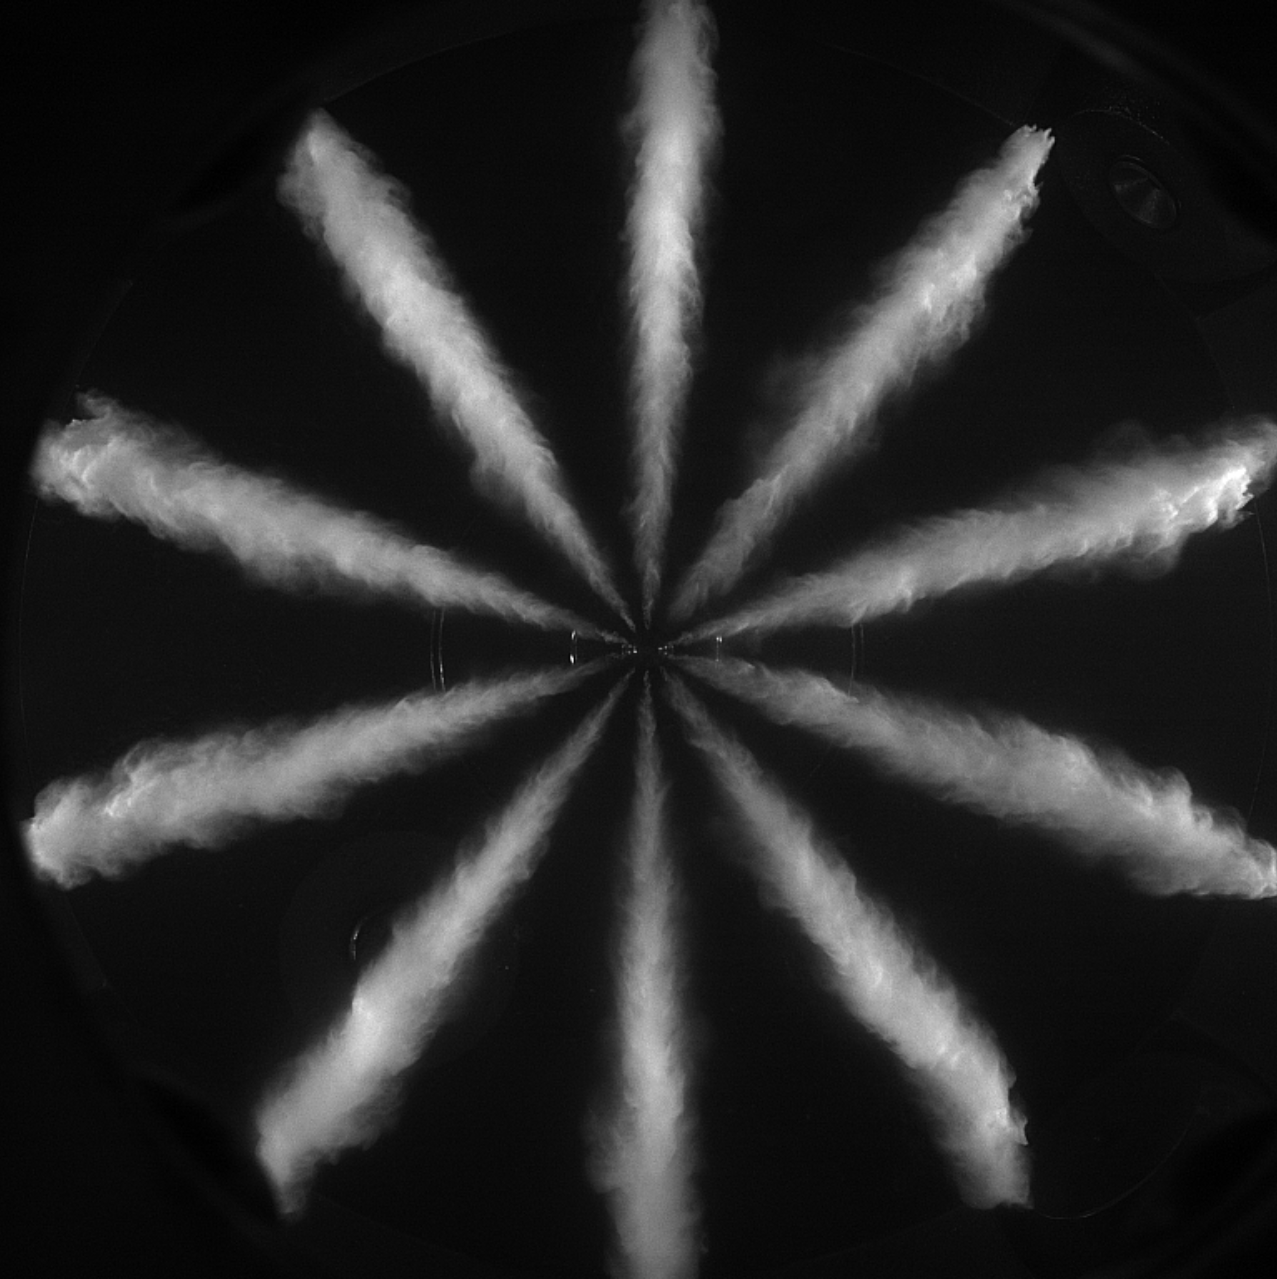
\includegraphics[width=0.9\linewidth]{../images/right_censoring_example.png}
\caption{喷雾图像中的右删失实例。部分喷油束已越过观测窗口上边界，因此在上限附近仅留下模糊的环状边缘痕迹；另一些喷油束尚未超过观测边界，仍完整显示在可见窗口内。}
\label{fig:right-censoring-example-zh}
\end{figure}

这一区别对代理模型训练具有直接影响。
若将删失轨迹的可见端点当作普通回归标签，目标值会在本应继续增长的晚期区域被系统性压低。
模型因而可能被训练成将``离开视场''解释为``物理饱和''。
在删失与未删失轨迹混合的数据集中，这种标签构造会产生不稳定的晚期梯度，并将穿深曲线人为拉平。
此时问题不在于模型表达能力不足，而在于监督信号本身已经存在偏差。

从统计建模角度看，Tobit 模型是处理删失因变量的经典起点 \cite{Tobin1958}。
如果本文的目标只是预测某一固定时刻的删失标量，Tobit 类型回归自然是值得优先考虑的基线。
然而，本文面对的并非单个标量，而是受 SOI、EOI 与喷嘴瞬态共同塑造的短时穿深轨迹。
对于已经越过视场边界的晚期样本，Tobit 似然主要提供``真实值高于删失边界''的单侧约束，
而不能提供``越界之后轨迹应如何继续增长''的形状信息。
当晚期未删失样本本就稀少且保守外推不可避免时，这类梯度更容易帮助模型学习``是否越界''，
却不足以稳定恢复``越界后延拓到何种程度''。
就本文的数据条件而言，这种信息结构并不适合作为晚期轨迹重建的主要依据。

不确定性感知扩展的动机在于，并非每个工况点或每条提取轨迹都具有相同可信度。
异方差高斯负对数似然是一种标准做法，可使网络同时预测均值与输入相关方差 \cite{KendallGal2017}。
在回归形式上，它对应条件模型
\[
y=\mu(x,t)+\varepsilon(x,t),\qquad \varepsilon(x,t)\sim \mathcal{N}(0,\sigma^2(x,t)),
\]
这里的高斯分布应理解为实用统计假设，而非声称喷雾物理在每个瞬间均真实服从高斯分布 \cite{BishopPRML2006,KendallGal2017}。
本文真正需要的是一种表达未解析因素合成残差的方式，并将该残差与条件均值轨迹区分开来；
否则，模型将被迫把所有 plume 间和循环间差异都压入单一均值函数中。

然而，仅依靠异方差回归并不能完全消除右删失导致的系统性低估。
若直接使用原始部分观测轨迹进行监督，即便网络能够输出方差，其晚期均值仍可能被视场边界向下拉偏。
因此，本文进一步采用教师引导的蒸馏式细化：
首先在前述``人工拟合并保守外推''的合成轨迹上训练异方差教师模型，使其学习删失感知的晚期延拓；
随后利用该教师模型约束面向原始 CDF 观测的学生模型。
在这一框架中，可靠的早中期原始观测仍保留直接监督地位，而晚期稀疏或已删失区间则更多依赖教师提供的软目标。
换言之，蒸馏在本文中并非一般意义上的模型压缩技巧，而是将删失感知合成数据重新投射回原始观测域的偏差修正机制。

高斯输出在此还具有一个实际优势：
当教师和学生都输出单变量高斯分布时，两者之间的 Kullback--Leibler 散度有解析闭式解：
\[
D_{\mathrm{KL}}\!\left(\mathcal{N}(\mu_1,\sigma_1^2)\,\|\,\mathcal{N}(\mu_2,\sigma_2^2)\right)
=\log\frac{\sigma_2}{\sigma_1}+\frac{\sigma_1^2+(\mu_1-\mu_2)^2}{2\sigma_2^2}-\frac{1}{2},
\]
这意味着蒸馏损失可以精确计算，无需蒙特卡洛采样，也不会向训练过程额外引入梯度方差
\cite{BishopPRML2006,KendallGal2017}。
KL 方向本身仍然是一个需要说明的设计选择。
本文保留 forward KL，即以学生分布近似教师分布，因为它与 Stage~1--2 已采用的负对数似然目标形式一致，并且在稀疏晚期样本处更偏向覆盖教师分布的整体质量。
相比之下，reverse KL 更偏向锁定教师分布的主峰，对细薄尾部和少数外推轨迹不够敏感。
在本文关心的工况范围内，两种方向的预测差异经初步检查较小；因此 forward KL 应被理解为有意选择但尚未通过完整消融单独证明的保守设计。
近期关于回归蒸馏与不完整监督的研究也表明，教师软目标可以在直接标签缺失或不可靠区域显著降低学生误差
\cite{HintonVinyalsDean2015,TarvainenValpola2017,KangKang2024KDRegression}。

综上，本文真正重要的并不是将网络划分为若干训练阶段，而是将三项设计绑定在同一学习框架中：
右删失感知的数据构造、输入相关不确定性的异方差回归，以及基于人工拟合与外推教师的蒸馏式偏差修正。
三者共同服务于同一目标：
避免模型将``离开视场''误学为``停止生长''。

\subsection{形状约束与物理信息神经网络}

除右删失和不确定性之外，代理模型还需要满足最基本的穿深形状约束。
纯数据驱动的平滑 MLP 在样本密集区域通常能给出合理插值；
但在局部稀疏或轻度外推的工况空间中，模型可能出现没有物理依据的振荡、局部回退或尖锐梯度。
本文测试矩阵中确实存在此类支持较弱的局部区域，例如特定喷孔直径、喷射压力和持续时间组合。
因此，仅依靠数据损失并不足以保证轨迹形状始终可信。

将物理先验写入神经网络训练，是物理信息神经网络（Physics-Informed Neural Networks, PINNs）文献中的代表性思路 \cite{Raissi2019PINNs}。
Raissi 等工作的核心机制在于：利用自动微分（Automatic Differentiation）计算网络输出相对于输入的偏导数，
并将这些导数相关项作为软惩罚加入损失函数。
这样，偏微分方程或经验物理规律便可作为约束，引导网络在数据稀疏区域仍停留在较合理的函数空间内。

本文并不试图用神经网络求解完整的 Navier--Stokes 方程。
这里借用的是 PINNs 的约束思想：
通过自动微分得到穿深均值对时间的一阶和二阶导数，并在损失中加入相应的软惩罚。
一阶导数约束用于抑制不合理的负速度，二阶导数约束用于鼓励喷射及喷射后减速阶段整体呈现凹性，即穿深增长率随时间衰减。
这也解释了为何前文提到的 Swish/SiLU 等平滑激活函数是必要的：
只有当二阶导数能够稳定、平滑地传递，基于曲率的物理形状约束才适合用梯度下降优化。

\subsection{概率预测的评估：适当评分规则与模型校准}

让网络同时输出均值和方差，并不自动意味着它的不确定性就是可靠的。
概率预测的评价标准与确定性回归不同：
均方误差或平均绝对误差主要评价点预测，而预测分布还必须同时接受精度和离散度的检验。
因此，评估概率模型需要使用严格适当评分规则（Strictly Proper Scoring Rules）。
Gneiting 和 Raftery 的工作表明，只有当预测分布与真实条件分布一致时，适当评分规则才会达到其期望最优值 \cite{GneitingRaftery2007CRPS}。
连续排位概率分数（Continuous Ranked Probability Score, CRPS）是其中常用的一类指标：
它同时惩罚均值偏差和预测分布过宽，使模型既要准确，也要保持适当的锐度。

此外，现代深度网络即使点预测精度较高，也可能出现过度自信：
预测区间的标称概率并不一定等于真实观测落入该区间的经验频率。
Guo 等对这一现象进行了系统诊断，并强调事后概率校准与经验覆盖率检查的必要性 \cite{Guo2017Calibration}。
在本文场景中，单纯训练得到的异方差网络可能在某些工况下给出过小的方差，
导致实际观测值落出预测区间的频率高于标称水平。
因此，面向早期设计筛查的代理模型必须在留出集上检验不确定度校准；
对于分布外泛化，还应通过留出完整硬件族等空间交叉验证检查经验覆盖率，例如 $1\sigma$ 和 $2\sigma$ 覆盖率。
这也构成了后文结果评估中采用 CRPS、可靠性图和留一喷嘴族（OOD）诊断的依据。

\subsection{喷雾撞壁机理与概率性碰撞风险筛查}

柴油预喷喷雾的穿深控制首先是一项燃烧组织问题，而不仅仅是撞壁规避问题。
在双燃料柴油-气体发动机中，预喷喷雾的几何分布——包括穿深、锥角与液相延伸范围——直接决定点火核的空间位置与尺寸，
并由此影响火焰能否高效传播至预混的主燃料气体充量
\cite{Karim2015DualFuel,WeiGeng2016DualFuelReview,Sahoo2009DualFuelReview}。
若预喷穿深过短，点火核位置偏离合适区域或体积不足，可能导致主燃料火焰传播不充分、未燃碳氢化合物（如甲烷滑漏）升高，整体燃烧效率随之下降；
若预喷穿深过长，则即便尚未发生明确撞壁，也可能改变点火核与气体充量的相对位置，导致主燃料燃烧不充分，并增加液相撞壁的可能性
\cite{WeiGeng2016DualFuelReview,Sahoo2009DualFuelReview}。
换言之，预喷穿深首先是主燃料混合、点火核布置和燃烧效率的关键控制变量；
在此基础上，它也是撞壁风险筛查的几何核心输入。
本文对预喷穿深及其不确定性的预测因此优先服务于预喷控制与燃烧组织评估，同时也服务于壁面风险排序。

当这一空间控制失效时，液相喷雾与发动机壁面的接触才成为必须处理的后果之一。
若液态燃料在蒸发或点火之前到达活塞顶或缸壁，壁面上可能形成燃油液膜，并造成壁面润湿、局部混合恶化、未燃碳氢排放升高以及机油稀释
\cite{peraza2022swi,ahmad2025fueldilution,MorieiraMotaPanao2010}。
该问题不能仅从单液滴碰壁的微观物理角度理解。
Moreira 等在综述中指出，单液滴撞击研究确实积累了大量基础知识，
但将其直接外推至连续喷雾撞壁并不稳妥，因为喷雾 plume 的集体行为还受到邻近液滴相互作用、残余壁膜和二次雾化等因素调制
\cite{MorieiraMotaPanao2010}。
因此，从单液滴到 plume 并非简单平滑插值，而存在真实尺度与机理缺口。
在船用大缸径尺度下，问题进一步复杂化：
喷雾发展尺度并不能通过简单比例放大获得，针对大型海用喷嘴的光学研究也表明，壁面约束会显著改变点火延迟和自然发光火焰强度
\cite{liu2024marine_impingement}。

工程上最直接的筛查规则相对明确：
比较液相尖端穿深 $S_\mathrm{tip}(t)$ 与喷嘴到壁面的距离 $L_\mathrm{wall}$，当 \(S_\mathrm{tip}(t) \geq L_\mathrm{wall}\) 时标记为撞壁
\cite{Baumgarten2006MixFormation}。
Baumgarten 关于内燃机混合气形成的系统论述中，也把穿深关联式视为简化喷雾轨迹的基线工具，并把穿深与壁距比较作为一阶撞壁判据
\cite{Baumgarten2006MixFormation}。
值得指出的是，后续研究并未抛弃这一几何核心，而是在其基础上补充更多信息。
Park 等针对高压汽油直喷，从喷雾图像重建径向燃油质量分布，
并结合喷射时序估算撞击活塞和缸壁的燃油质量份额；
其趋势结论，即喷射压力升高、雾化增强时撞壁量下降，本身并不意外，更有价值的是其方法论含义：
图像分析可以在不进行完整 CFD 的条件下给出定量撞壁估计
\cite{Park2018WallImpingement}。
ECN 框架下，Peraza 等人使用单孔喷嘴和受控温度平板壁面系统测量喷雾撞壁，刻画了穿深-壁距关系如何随环境密度和温度变化
\cite{peraza2022swi}。
这些工作共同说明：
无论测量细节如何变化，穿深仍是撞壁筛查中最关键的几何输入。

然而，对于短脉冲预喷而言，将确定性阈值作为主要筛查工具过于脆弱。
穿深本身带有来自针阀瞬态、循环间动量波动和残余光学测量噪声的不确定性；SOI/EOI 主导的阶段又使稳态关联式在大段观测窗口内不够可靠。
若将本应被视为分布的量压缩为单一数值，再进行二值 pass/fail 判断，会隐藏对候选工况排序有用的信息。
本文的处理方式是将穿深表示为条件高斯分布 \(S_\mathrm{tip}\sim\mathcal{N}(\mu(x,t),\,\sigma^2(x,t))\)，并把该分布投影到以喷嘴中心为原点的二维发动机几何平面。
在横向扩展由喷雾半锥角控制、并以正态分布近似的前提下，喷雾前沿的概率密度可写成旋转二维高斯。
在这一简化几何下，撞壁风险分数可表示为该分布落入壁面和活塞几何掩膜区域内的概率质量积分。
该输出应被理解为面向早期设计排序的概率性筛查代理指标，而非经过完整验证的生产级撞壁预测。

\begin{table}[t]
\centering
\footnotesize
\setlength{\tabcolsep}{2pt}
\renewcommand{\arraystretch}{1.12}
\begin{tabular}{@{}L{0.20\linewidth}L{0.25\linewidth}L{0.25\linewidth}L{0.23\linewidth}@{}}
\toprule
文献脉络 & 支撑内容 & 对本文仍不足 & 本文响应 \\
\midrule
Mie 光学诊断与几何观测量 & 强度可支撑穿深、锥角、边界等几何观测量；ECN 等基准研究确认光学度量是方法依赖的。 & 强度不是液体体积分数或质量场的直接测量，且穿深定义随后处理规则变化。 & 将输出解释为边界明确的光学液相包络度量，并在结果讨论中保留方法依赖性提示。 \\
喷雾穿深物理与短脉冲瞬态 & 经典与瞬态穿深律说明穿深具有明确物理意义并随阶段切换。 & 短预喷可观测窗口同时包含 SOI、EOI 和喷嘴硬件时间尺度，单一刚性关联式难以覆盖整条轨迹。 & 采用柔性降阶目标和物理缩放，而非单一刚性关联式。 \\
CUDA 并行图像处理与多孔配准 & 标定、对数预处理、梯度、极坐标映射、傅里叶配准与鲁棒拟合都有成熟依据。 & 没有单一现成方法覆盖完整多孔视频工作流，单射流分割工具不能稳定配准重复喷油束。 & 以标准、可检查的算子组成可审计处理链，并以喷嘴中心极坐标和喷油束对齐坐标利用对称性。 \\
数据驱动代理模型与删失/不确定性 & ANN/MLP 类模型已可预测喷雾宏观量；删失统计与异方差/教师蒸馏均为成熟工具。 & 既有喷雾代理模型工作较少把视场损失显式当作右删失，也较少把输入相关不确定性作为一等输出。 & 引入删失感知目标构造、异方差 NLL 与教师引导蒸馏，三者整合在同一学习框架中。 \\
物理信息学习与形状约束 & 自动微分可将物理导数约束写入神经网络训练目标。 & 稀疏工况下，纯数据驱动模型可能产生非物理振荡；本文也不需要求解完整 PDE。 & 用一阶和二阶时间导数软惩罚约束穿深轨迹形状。 \\
撞壁风险筛查 & 穿深与壁距比较仍是一阶撞壁判据的核心几何输入。 & 确定性阈值在强瞬态、高不确定性条件下易掩盖排序所需信息。 & 输出条件高斯穿深，并通过简化二维几何投影给出概率性撞壁代理指标。 \\
\bottomrule
\end{tabular}
\caption{既有文献脉络及其在本文中的设计响应。}
\label{tab:literature-synthesis-zh}
\end{table}

综上，现有文献为本文提供了表~\ref{tab:literature-synthesis-zh} 所概括的支撑线索。
Mie 散射理论说明了光学强度为何只能被谨慎转化为几何观测量；
计算机视觉和信号处理理论支撑了图像处理链中的各个局部步骤，即使没有一个现成工具能够直接覆盖整条流程；
柴油喷雾物理明确了穿深和锥角作为描述符的意义，也同样明确了它们的解释边界；
ECN 基准研究将光学度量的方法依赖性明确呈现出来；
已有 ANN/MLP 代理模型研究说明喷雾宏观量的快速回归预测本身是可行的，但尚未自然解决短脉冲部分观测轨迹的偏置问题；
物理信息学习文献提供了通过自动微分写入导数约束的通用机制；
喷雾撞壁文献则确认了穿深作为几何筛查输入的中心地位，同时暴露出确定性阈值在强瞬态、高不确定性条件下的脆弱性。

仍需指出的是，没有任何单一文献脉络同时处理本文面对的组合问题：
（1）短脉冲预喷中 SOI 和 EOI 瞬态主导可观测窗口；
（2）有限视场使训练目标发生系统性右删失；
（3）多孔喷嘴要求围绕喷油束几何定制配准和提取流程，而不能将单孔工具事后套用；
（4）学习框架需要整合删失感知合成目标、异方差回归与教师蒸馏，以避免把观测截断误学成物理饱和；
（5）稀疏工况下还需要用导数软约束抑制非物理轨迹形状；
（6）预测得到的条件高斯穿深还需映射至简化发动机几何掩膜，形成适合早期设计筛查的概率性风险代理指标。
本文的贡献不在于分别触及这些问题，而在于将其作为同一工作流的设计约束加以处理。
后续章节将进一步检验这一整合方案是否成立。
